\title{Solving Quantum Anharmonic Osciallators Numerically}
\author{
        Kevin Belleville \\
        University of California, Los Angeles\\
        Physics 188B, Josh Samani\\
}
\date{\today}

\documentclass[12pt]{article}

\usepackage{braket}
\usepackage[margin=1in]{geometry}
\usepackage{graphicx}
\usepackage{float}

\begin{document}
\maketitle

\begin{abstract}
We apply our knowledge of the quantum harmonic oscillator to approximately numerically diagonalize and analyze the quantum anharmonic oscillator.
\end{abstract}

\section{Introduction}

\subsection*{The Quantum Harmonic Oscillator}

The Hamiltonian of the quantum harmonic oscillator is:

\begin{equation}
\hat{H_0} = \frac{1}{2} ( \hat{p}^2 + \hat{x}^2 )
\end{equation}

where $\hat{x}$ and $\hat{p}$ satisfy the canonical commutation relation:

\begin{equation}
[ \hat{x} , \hat{p} ] = i
\end{equation}

where $\hbar = 1$. We can diagonalize the Hamiltonian by introducing a raising operator $\hat{a}_+$ and a lowering operator $\hat{a}_-$.

\begin{equation}
\hat{a}_+ = \frac{1}{\sqrt{2}} ( \hat{x} - i \hat{p} )
\end{equation}

\begin{equation}
\hat{a}_- = \frac{1}{\sqrt{2}} ( \hat{x} + i \hat{p} )
\end{equation}

Using this new notation, we can redefine the Hamiltonian in terms of them as such:

\begin{equation}
\bar{H_0} = \hat{a}_+ \hat{a}_- + \frac{1}{2} I
\end{equation}

where $I$ is simply the identity matrix. There exists an orthonormal basis:

\begin{equation}
B_0 = \{ \ket{0}, \ket{1}, \ldots \}
\end{equation}

for the Hilbert space of the system such that:

\begin{equation}
\hat{a_+} \ket{n} = \sqrt{n+1} \ket{n+1}
\end{equation}

\begin{equation}
\hat{a_-} \ket{n} = \sqrt{n} \ket{n-1}
\end{equation}

This allows us to compute $\hat{H_0} \ket{n}$ as

\begin{equation}
\hat{H_0} \ket{n} = \left(n + \frac{1}{2}\right) \ket{n}
\end{equation}

Since the Hamiltonian is diagonal in the basis, the eigenvalues $E_n$ corresponding to the eigenvector $\ket{n}$ is

\begin{equation}
E_n = n + \frac{1}{2}
\end{equation}

To compute the matrix elements of the Hamiltonian, we apply a bra $\bra{m}$:

\begin{equation}
\bra{m} \hat{H_0} \ket{n} = \left( n + \frac{1}{2} \right) \delta_{mn}
\end{equation}

where $\delta_{ij}$ is the Dirac delta function. The Dirac delta function evaluates to 1 when $i = j$, otherwise it evaluates to 0. The raising and lowering operators can create matrix representations just like the Hamiltonian with the following expressions:

\begin{equation}
\bra{m} \hat{a_+} \ket{n} = \sqrt{n+1} \delta_{m, n+1}
\end{equation}

\begin{equation}
\bra{m} \hat{a_-} \ket{n} = \sqrt{n} \delta_{m, n-1}
\end{equation}

\section{Assignment 1}
\paragraph{Show that the operators $\hat{x}^2$ and $\hat{x}^4$ have the following matrix elements in the harmonic oscillator basis.} 

Using the raising and lowering operators are the obvious way to go, but first one must define the operator $\hat{x}$ in terms of $\hat{a_+}$ and $\hat{a_-}$.

\begin{equation}
\hat{x} = \frac{1}{\sqrt{2}} ( \hat{a_+} + \hat{a_-} )
\end{equation}

Since $\hat{x}^2$ is the operator acting on itself, it can be written as:

\begin{equation}
\hat{x}^2 = \frac{1}{2}  ( \hat{a_+} + \hat{a_-} )^2 = \frac{1}{2} ( \hat{a_+} \hat{a_+} + \hat{a_-} \hat{a_+} + \hat{a_+} \hat{a_-} + \hat{a_-} \hat{a_-} )
\end{equation}

With the matrix representation:

\begin{equation}
\bra{n} \hat{x}^2 \ket{m}= \frac{1}{2} ( \bra{n}\hat{a_+} \hat{a_+}\ket{m} + \bra{n}\hat{a_-} \hat{a_+}\ket{m} + \bra{n}\hat{a_+} \hat{a_-}\ket{m} + \bra{n}\hat{a_-} \hat{a_-} \ket{m})
\end{equation}

When dealing with operators, one must be sure to remember that order matters, as in $\hat{a_-} \hat{a_+}$ and $\hat{a_+} \hat{a_-}$ are not the same, and cannot be combined as if they were regular terms. Since these terms will be showing up a lot for the next operator calculation $\hat{x}^4$, it would be wise to explicitly state the values of their matrix representations to make the algebra a bit easier to understand. 

\begin{equation}
\hat{a_-} \hat{a_+} \ket{n} = (n+1) \ket{n}
\end{equation}

\begin{equation}
\hat{a_+} \hat{a_-} \ket{n} = n \ket{n}
\end{equation}

Now, back to the operator at hand, $\hat{x}^2$. We have already essentially figured out the middle two terms, but the outer terms must be brute forced, using the definitions in the Introduction.

\begin{equation}
\hat{a_+} \hat{a_+} \ket{n} =  \sqrt{(n+1)(n+2)} \ket{n+2}
\end{equation}

\begin{equation}
\hat{a_-} \hat{a_-} \ket{n} = \sqrt{n ( n- 1)} \ket{n-2}
\end{equation}

Substituting these calculated values into the original equation, and applying Dirac's delta function, we find that our matrix representation is:

\begin{equation}
\bra{n} \hat{x}^2 \ket{m} = \left( n + \frac{1}{2} \right) \delta_{nm} +
							\frac{1}{2} \sqrt{(n+1)(n+2)} \delta_{n, m-2} +
							\frac{1}{2} \sqrt{(n-1) n} \delta_{n, m+2}
\end{equation}

For the case of the $\hat{x}^4$ operator:

\begin{equation}
\hat{x}^4 = \frac{1}{4} ( \hat{a_+} + \hat{a_-} )^4
\end{equation}

\begin{equation}
\bra{n} \hat{x}^4 \ket{m} = \frac{1}{4} \bra{n}( \hat{a_+} + \hat{a_-} )^4 \ket{m}
\end{equation}

One can quickly realize that there will be 16 terms in this polynomial, none of which can be concatenated to one another to reduced the load. However, one can also realize that these terms can be separated into different groups, based on their Dirac delta functions. The delta functions depend on the number of raising and number of lowering operators, specifically. Take the previous calculations as an example. The first term with $\delta_{nm}$ is a combination of the two terms that had ONE raising and ONE lowering operator. The second term is TWO raising and ZERO lowering, while the third is ZERO raising and TWO lowering. \\
							 
For the case of $\hat{x}^4$, there will be five terms. One term will be FOUR raising, ZERO lowering; the next will be ZERO raising and FOUR lowering. These terms only have one permutation each, so they will only have one term. \\

For the case of THREE raising and ONE lowering, there are four possible permutation, which will all add together with a unique delta function. The same can be said for the case of ONE raising and THREE lowering. \\

The last case is where there are TWO raising and TWO lowering; there will be six different terms for this. I also can't exactly get the entire expanded polynomial to output onto \LaTeX, so I will do each term separately, and the pattern will be obvious.

\subsection*{FOUR Raising, ZERO Lowering}

Recall that to compute brakets with more than one operator, one begins with the right-most operator and works one's way to the right. I will be pulling the constants out to the left to make things clearer.

\begin{equation}
\bra{n} \hat{a_+}\hat{a_+}\hat{a_+}\hat{a_+} \ket{m} = \sqrt{m+1}\bra{n} \hat{a_+}\hat{a_+}\hat{a_+} \ket{m + 1}
\end{equation}

\begin{equation}
= \sqrt{(m+1)(m+2)}\bra{n} \hat{a_+}\hat{a_+}\ket{m + 2}
\end{equation}

One can begin to notice a pattern, and calculating the final result is:

\begin{equation}
\sqrt{(m+1)(m+2)(m+3)(m+4)}\braket{n|m + 4}
\end{equation}

The braket $\braket{n|m + 4}$ evaluates to the delta function $\delta_{n, m+4}$. This equation only exists where $n = m+4$, so we can redefine the result in terms of $n$ as such: (also include the $1/4$ constant from the beginning)

\begin{equation}
\frac{1}{4}\sqrt{ (n-3) (n-2) (n-1) n } \delta_{n, m+4}
\end{equation}

\subsection*{ZERO Raising, FOUR Lowering}

Using the same steps described above, one can calculate the result.

\begin{equation}
\bra{n} \hat{a_-}\hat{a_-}\hat{a_-}\hat{a_-} \ket{m} = \frac{1}{4}\sqrt{ (n+1) (n+2) (n+3) (n+4) } \delta_{n, m-4}
\end{equation}

\subsection*{THREE Raising, ONE Lowering}

There are four possible permutations of this.

\begin{equation}
\bra{n} \hat{a_+}\hat{a_+}\hat{a_+}\hat{a_-} \ket{m} 
\end{equation}

\begin{equation}
\bra{n} \hat{a_+}\hat{a_+}\hat{a_-}\hat{a_+} \ket{m} 
\end{equation}

\begin{equation}
\bra{n} \hat{a_+}\hat{a_-}\hat{a_+}\hat{a_+} \ket{m} 
\end{equation}

\begin{equation}
\bra{n} \hat{a_-}\hat{a_+}\hat{a_+}\hat{a_+} \ket{m} 
\end{equation}

All end up with the same delta function $\delta_{n, m+2}$, so let's focus on the values that are computed. Begin with the top most equation, we use a trick. Since we know that:

\begin{equation}
\hat{a_+} \hat{a_-} \ket{n} = n \ket{n}
\end{equation}

we can use it as a shortcut. Applying this to the right-most operators, the equation becomes:

\begin{equation}
\bra{n} \hat{a_+}\hat{a_+}\hat{a_+}\hat{a_-} \ket{m}  = 
m \bra{n} \hat{a_+}\hat{a_+} \ket{m}
\end{equation}

\begin{equation}
m \bra{n} \hat{a_+}\hat{a_+} \ket{m} = m \sqrt{ (m+1) (m+2) } \bra{n}\ket{m+2} = 
m \sqrt{ (m+1) (m+2) } \delta_{n, m+2}
\end{equation}

Solving for $n$, since the equation only evaluates when $n = m+2$:

\begin{equation}
(n-2) \sqrt{ (n-1) n} \delta_{n, m+2}
\end{equation}

Solving for the next:

\begin{equation}
\bra{n} \hat{a_+}\hat{a_+}\hat{a_-}\hat{a_+} \ket{m} = \sqrt{m+1} \bra{n} \hat{a_+}\hat{a_+}\hat{a_-} \ket{m + 1}
\end{equation}

\begin{equation}
 = (m+1) \sqrt{ (m+1) (m+2) } \delta_{n, m+2}
\end{equation}

\begin{equation}
(n-1) \sqrt{ (n-1) n} \delta_{n, m+2}
\end{equation}

One can notice that there is a pattern in these results. The position of our shortcut is the only thing that changes throughout these calculations, and that changes $n-2$ to $n-1$. We can extrapolate that the next two will be $n$ and $n+1$. (I verified this by hand.) This means that:

\begin{equation}
\bra{n} \hat{a_+}\hat{a_-}\hat{a_+}\hat{a_+} \ket{m} = 
(n) \sqrt{ (n-1) n} \delta_{n, m+2}
\end{equation}

\begin{equation}
\bra{n} \hat{a_-}\hat{a_+}\hat{a_+}\hat{a_+} \ket{m} = 
(n+1) \sqrt{ (n-1) n} \delta_{n, m+2}
\end{equation}

Summing all four of these results together, and including the $1/4$ factor from before, we find that the term for this delta function is:

\begin{equation}
\frac{1}{4}( n - 2 + n - 1 + n + n + 1 ) \sqrt{ (n-1) n} \delta_{n, m+2}
\end{equation}

\begin{equation}
\frac{1}{4}(4n - 2) \sqrt{ (n-1) n} \delta_{n, m+2}
\end{equation}

\begin{equation}
\left(n - \frac{1}{2}\right) \sqrt{ (n-1) n} \delta_{n, m+2}
\end{equation}

\subsection*{ONE Raising, THREE Lowering}

Using the method described above, these four terms can be calculated and summed together to:

\begin{equation}
\left( n + \frac{3}{2} \right) \sqrt{ (n+1) (n+2) } \delta_{n, m-2}
\end{equation}

\subsection*{TWO Raising, TWO Lowering}

The six terms can be computed quickly using tricks picked up from the previous methods:

\begin{equation}
\bra{n} \hat{a_+} \hat{a_-} \hat{a_+}  \hat{a_-}  \ket{m} = n^2 \delta_{nm}
\end{equation}

\begin{equation}
\bra{n} \hat{a_-}\hat{a_+} \hat{a_-} \hat{a_+}    \ket{m} = (n+1)^2 \delta_{nm}
\end{equation}

\begin{equation}
\bra{n} \hat{a_+}  \hat{a_+} \hat{a_-}  \hat{a_-} \ket{m} = (n-1) n \delta_{nm}
\end{equation}

\begin{equation}
\bra{n} \hat{a_-}\hat{a_-}\hat{a_+}  \hat{a_+}    \ket{m} = (n+2)(n+1) \delta_{nm}
\end{equation}

\begin{equation}
\bra{n} \hat{a_+} \hat{a_-}\hat{a_-} \hat{a_+}    \ket{m} = n(n+1)\delta_{nm}
\end{equation}

\begin{equation}
\bra{n} \hat{a_-}\hat{a_+}  \hat{a_+} \hat{a_-}   \ket{m} = n(n+1)\delta_{nm}
\end{equation}

Summing together the beginning terms:

\begin{equation}
n^2 + (n+1)^2 + (n-1) n + (n+2)(n+1) + n(n+1) + n(n+1) = 6n^2 + 6n + 3
\end{equation}

Thus, the whole term including the $1/4$ is:

\begin{equation}
\frac{1}{4} (6n^2 + 6n + 3) \delta_{nm}
\end{equation}

\subsection*{All Terms Together}

Adding up all of these terms yields the result:



$$ \bra{n} \hat{x}^4 \ket{m}  =\frac{1}{4} (6n^2 + 6n + 3) \delta_{nm}  +  \\
						 \left( n + \frac{3}{2} \right) \sqrt{ (n+1) (n+2) }   \delta_{n, m-2}   +  \\ $$ $$ 
					 \left(n - \frac{1}{2}\right) \sqrt{ (n-1) n} \delta_{n, m+2}  +  \\ 
						 \frac{1}{4}\sqrt{ (n+1) (n+2) (n+3) (n+4) } \delta_{n, m-4}  + \\ $$ 
						$$ \frac{1}{4}\sqrt{ (n-3) (n-2) (n-1) n } \delta_{n, m+4}$$ 
						
\section{Assignment 2}

\paragraph{Solve the anharmonic oscillator eigenvalue problem written in the harmonic oscillator basis for at least the first four energy levels.}

The Hamiltonian for the anharmonic oscillator can be defined in terms of the harmonic oscillator's Hamiltonian, with an extra term, as presented below:

\begin{equation}
\hat{H}_{\lambda} = \hat{H}_0 + \lambda \hat{x}^4
\end{equation}

To solve for the energy eigenvalues, we must convert this form into:

\begin{equation}
\hat{H}_{\lambda} \ket{n} = \hat{H}_0 \ket{n}+ \lambda \hat{x}^4 \ket{n}
\end{equation}

Which can be expanded into:

\begin{equation}
\hat{H}_{\lambda} \ket{n} = \left( n+ \frac{1}{2} \right) \ket{n}+ \lambda \hat{x}^4 \ket{n}
\end{equation}

where the term $\hat{x}^4 \ket{n}$ is actually a form of the gigantic expression we just defined in Assignment 1. Obviously, this is nearly impossible to do analytically, but we can do this numerically. I will utilize a optimized eigenvalue solver to compute this. The first four eigenvalues of the anharmonic oscillator with $\lambda = 1$ and basis size of $N=100$ are:

\begin{equation}
E_0' = 0.804    
\end{equation}
\begin{equation}
E_1' =    2.738
\end{equation}
\begin{equation}
E_2' =      5.179    
\end{equation}
\begin{equation}
E_3' =       7.942
\end{equation}

If we set $\lambda = 0.01$, much smaller, we can see the resemblance between these eigen values and the harmonic's. They are all close to the original's values of $n+1/2$.        

\begin{equation}
E_0' = 0.507    
\end{equation}
\begin{equation}
E_1' =   1.536
\end{equation}
\begin{equation}
E_2' =       2.591    
\end{equation}
\begin{equation}
E_3' =        3.671
\end{equation}



\section{Assignment 3}

\paragraph{Plot the first four energy levels versus $\lambda$ over the range $0 \leq  \lambda \leq 1$. Plot also the spacings between the levels $\Delta E(\lambda)$. Make sure to use a basis size $N$ larger than the desired number of lowest eigenvalues.} 

The graph below shows the energy eigenvalues as they change as $\lambda$ increases.

\begin{figure}[H]
\begin{center}
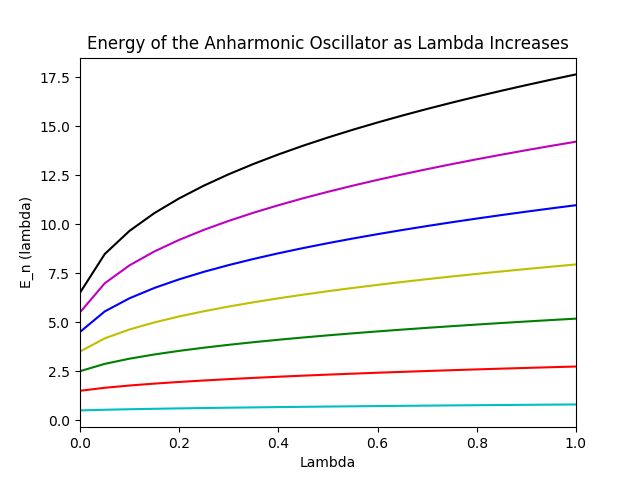
\includegraphics[scale=0.8]{energy_vs_lambda.png}
\end{center}
\end{figure}

One can look at the Hamiltonian of the anharmonic oscillator to understand that when $\lambda = 0$, it will be exactly the same as the Hamiltonian for the simple harmonic oscillator. There are 7 energy states shown in this figure, and the beginning of each one is when $\lambda = 0$ and thus each begins with $n+1/2$. We can see that the values begin at $0.5$, then $1.5$ and so on. However, as $\lambda$ increases, the $\hat{x}^4$ term overtakes the $\hat{H}_0$ term. We can also notice that this overtaking is not increasing at the same rate globally. For $n=0$, the energy level barely changes when $\lambda=0$ changes to $\lambda=1$. It does actually change, it just is not exactly visible on this scale. Nevertheless, we can note that lower energy levels are less affected by large changes in $\lambda$, whereas higher energy levels diverge rapidly. \\

To show the fact that this happens, the plot below shows the difference in energy levels with the equation $$ \Delta E(\lambda) = E_{n+1} (\lambda) - E_n (\lambda) $$.

\begin{figure}[H]
\begin{center}
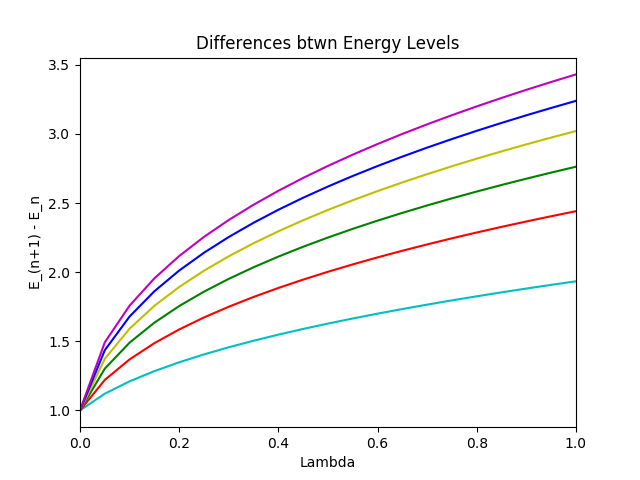
\includegraphics[scale=0.8]{diff_energy.png}
\end{center}
\end{figure}

I used the same color pattern as the plot above to demonstrate clarity. First, we can notice that at $\lambda=0$, all differences originate from 1. This is simply because the difference in energy would be $((n+1)+0.5) - (n + 0.5) = 1$. Next we can notice that the largest difference is in the zeroth and first energy levels, and they successively decrease afterward. One can expect that for energy levels greater than what I studied $(n-6)$, the difference would shrink further. This is logical based on what we know from our quantum mechanics classes.


\section{Assignment 4}

\paragraph{Check the convergence of the method with respect to the basis size $N$ by plotting one of the lowest energy eigenvalues $E_n(N)$ for $\lambda = 1$ versus the basis size $N$. You could also plot the differences between two consectuive estimates $\epsilon_n = E_n(N) - E_n(N+2)$ versus $N$.}

To demonstrate this, I used the lowest, most stable energy eigenvalue, $E_0$ with $\lambda = 1$. The approximated value for $E_0(N)$ is 0.83077.

\begin{figure}[H]
\begin{center}
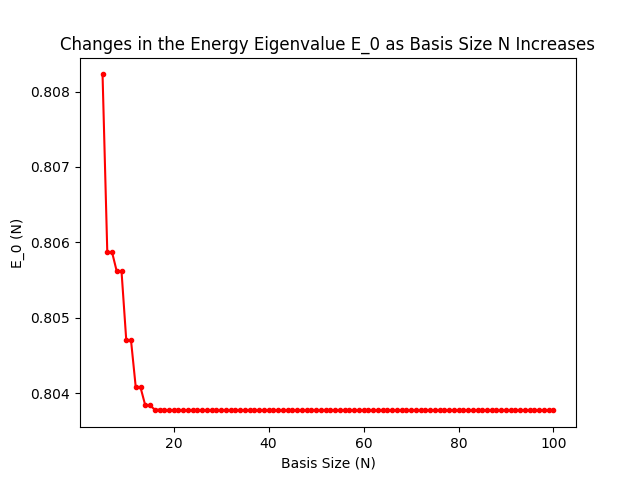
\includegraphics[scale=0.8]{basis.png}
\end{center}
\end{figure}

Notice that the graph converges quickly after a certain point, around $N=15$. After that, the changes are unnoticable, but before 15, the values are very off. I actually truncated the graph; it does not go from 1 to 100, but rather 5 to 100. The first couple values are so widely off, that I would not be able to show the most interesting part of the graph, such as at what N does the energy eigenvalue converge. One odd thing I noticed about my graph is that it does not oscillate below the expected value, and that there are some "double" points at which the basis sizes are $N$ and $N+1$, but the values are the same (at least from my point of view). I find that odd, and I'm not sure why that would be happening, save for some weird quirk in the eigenvalue generator I used.


\section{Assigment 5}

\paragraph{Plot and compare the first two eigenfunctions $\psi_n(x)$ for the harmonic oscillator with $\lambda = 0$ to the eigenfunctions for the anharmonic oscillators with $\lambda = 1$.}

The harmonic wavefunctions for the first four energy values are:

\begin{figure}[H]
\begin{center}
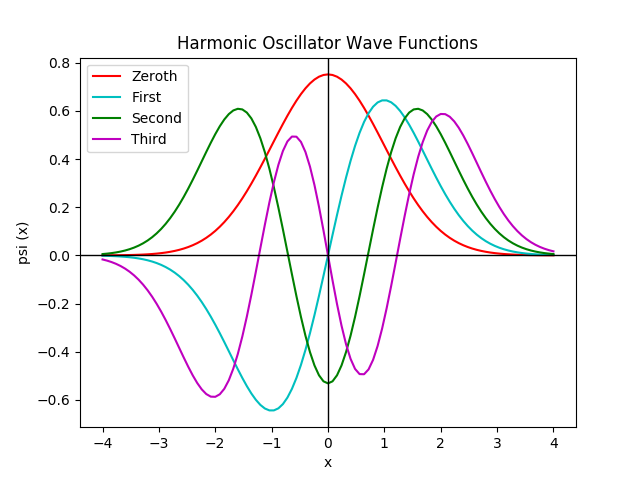
\includegraphics[scale=0.8]{harm_osc.png}
\end{center}
\end{figure}

The anharmonic wavefunctions for the same four are:

\begin{figure}[H]
\begin{center}
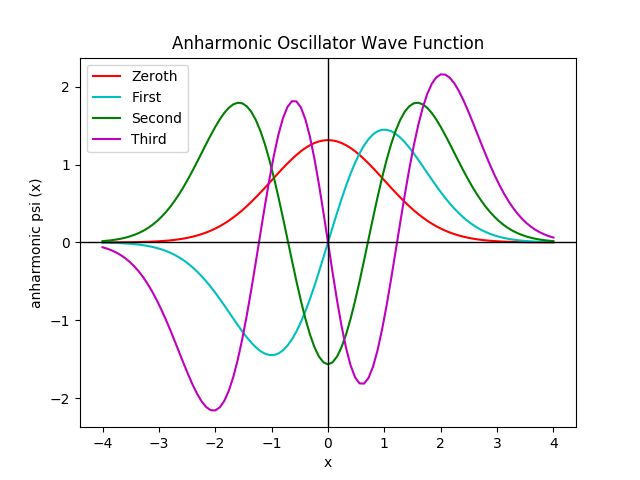
\includegraphics[scale=0.8]{anharm_osc.png}
\end{center}
\end{figure}

We can notice that the scale in the graphs is different. For the harmonic one, the max is around 0.8, whereas the max in the anharmonic one is nearly 2. We can tell that all wavefunctions increased, but the higher energy ones increased much more and overtook the bigger wavefunctions. This makes sense if one were to think about the equation for the anharmonic oscillator.

\section{Conclusions}
This project was a great review of the quantum harmonic oscillator, and a learning experience for things I have not yet learned, such as perturbation theory. There was a lot of algebra involved, but I feel like the work illuminated things about the concepts I had not solidified in my mind before. It was especially interesting how changing and basis size and $\lambda$ affected the energy levels. \\

Because of the fact that this is a relatively simple, solved problem in physics, I was rather surprised by the amount of work I had to do to learn how to compute it and learn all the intricacies of the quantum harmonic oscillator. It gave me an appreciation of how complicated real world systems are, and how mind-boggling complex the entire universe is. 



\begin{thebibliography}{9}

\bibitem{a} UCSC
\\\texttt{http://physics.ucsc.edu/~peter/242/anharmonic.pdf}

\bibitem{b} 
Journal of Undergraduate Research in Physics, 
\\\texttt{http://www.jurp.org/2012/MS134.pdf}

\bibitem{d} 
SciPy Documentation for method eigh,
\\\texttt{https://docs.scipy.org/doc/numpy-1.10.0/reference/generated/numpy.linalg.eigh.html}

\bibitem{e} 
jrjohansson on GitHub, 
\\\texttt{https://github.com/jrjohansson/wavefunction/blob/master/Wavefunction-Harmonic-Oscillator.ipynb}

\bibitem{f} 
Prof. Michael G. Moore, Michigan State University, 
\\\texttt{http://www.pa.msu.edu/~mmoore/TIPT.pdf}


\end{thebibliography}

\end{document}
